% Compile with XeLaTeX: xelatex main.tex (run twice for the table of contents)
\documentclass[11pt,a4paper]{article}

\usepackage[a4paper,margin=22mm,headheight=22pt]{geometry}
\usepackage{fontspec}
% Windows system fonts keep the report portable on the project environment.
\setmainfont{Times New Roman}
\setsansfont{Arial}
\usepackage{microtype}
\usepackage{setspace}
\usepackage{parskip}
\usepackage{graphicx}
\usepackage{float} % Provides [H] for non-floating figures
\usepackage{booktabs}
\usepackage{tabularx}
\usepackage{longtable}
\usepackage{array}
\usepackage{enumitem}
\usepackage{fancyhdr}
\usepackage{titlesec}
\usepackage{xcolor}
\usepackage{tcolorbox}
\usepackage{listings}
\usepackage{tikz}
\usetikzlibrary{arrows.meta,positioning,shapes.geometric,calc,fit}
\usepackage{hyperref}

\definecolor{Ink}{HTML}{172033}
\definecolor{InkMuted}{HTML}{5D677A}
\definecolor{Navy}{HTML}{0B1F3A}
\definecolor{Blue}{HTML}{176B87}
\definecolor{Teal}{HTML}{0E8A8A}
\definecolor{Accent}{HTML}{D97706}
\definecolor{SoftBlue}{HTML}{EAF3F8}
\definecolor{SoftTeal}{HTML}{E8F5F4}
\definecolor{SoftGray}{HTML}{F4F6F8}
\definecolor{Line}{HTML}{D7DEE8}

\hypersetup{
  colorlinks=true,
  linkcolor=Blue,
  urlcolor=Teal,
  citecolor=Blue,
  pdftitle={Hybrid FTP Application -- Technical Report},
  pdfauthor={Replace with team members}
}

\setstretch{1.12}
\setlength{\parindent}{0pt}
\setlist[itemize]{leftmargin=*,itemsep=2pt,topsep=3pt}
\setlist[enumerate]{leftmargin=*,itemsep=2pt,topsep=3pt}
\renewcommand{\arraystretch}{1.25}
\newcolumntype{Y}{>{\raggedright\arraybackslash}X}
\newcolumntype{P}[1]{>{\raggedright\arraybackslash}p{#1}}

\titleformat{\section}{\Large\bfseries\sffamily\color{Navy}}{\thesection.}{0.6em}{}
\titleformat{\subsection}{\large\bfseries\sffamily\color{Blue}}{\thesubsection}{0.6em}{}
\titleformat{\subsubsection}{\normalsize\bfseries\sffamily\color{Ink}}{\thesubsubsection}{0.6em}{}
\titlespacing*{\section}{0pt}{18pt}{8pt}
\titlespacing*{\subsection}{0pt}{13pt}{5pt}

\pagestyle{fancy}
\fancyhf{}
\lhead{\sffamily\small\textcolor{InkMuted}{Internetworking Protocols | Hybrid FTP}}
\rhead{\sffamily\small\textcolor{InkMuted}{Technical Report}}
\cfoot{\sffamily\small\textcolor{InkMuted}{\thepage}}
\renewcommand{\headrulewidth}{0.35pt}
\renewcommand{\headrule}{\hbox to\headwidth{\color{Line}\leaders\hrule height \headrulewidth\hfill}}

\newcommand{\placeholder}[1]{\textcolor{Accent}{\footnotesize\sffamily\textbf{[PH]}~#1}}
\newcommand{\code}[1]{\texttt{#1}}
\newtcolorbox{infobox}{colback=SoftBlue,colframe=Blue,boxrule=0.6pt,arc=1.5mm,left=3mm,right=3mm,top=2mm,bottom=2mm}
\newtcolorbox{placeholderbox}{colback=SoftGray,colframe=Accent,boxrule=0.7pt,arc=1.5mm,left=3mm,right=3mm,top=2mm,bottom=2mm}
\newcommand{\evidenceplaceholder}[2]{%
  \begin{figure}[H]
  \centering
  \fcolorbox{Accent}{SoftGray}{\parbox[c][42mm][c]{0.86\textwidth}{\centering\sffamily\textcolor{Accent}{\textbf{Screenshot placeholder}}\\[2mm]\textcolor{InkMuted}{#1}\\[3mm]\footnotesize Replace this box with #2.}}
  \caption{#1}
  \end{figure}%
}

\lstdefinestyle{reportcode}{
  basicstyle=\ttfamily\small,
  backgroundcolor=\color{SoftGray},
  frame=single,
  rulecolor=\color{Line},
  breaklines=true,
  columns=fullflexible,
  xleftmargin=2mm,
  xrightmargin=2mm,
  aboveskip=7pt,
  belowskip=7pt
}
\lstset{style=reportcode}

\tikzset{
  actor/.style={draw=Navy,fill=SoftBlue,rounded corners=2pt,minimum width=23mm,minimum height=8mm,align=center,font=\sffamily\small\bfseries},
  flow/.style={draw=Blue,fill=SoftBlue,rounded corners=2pt,minimum width=31mm,minimum height=8mm,align=center,font=\sffamily\scriptsize},
  state/.style={draw=Teal,fill=SoftTeal,rounded corners=2pt,minimum width=29mm,minimum height=8mm,align=center,font=\sffamily\scriptsize},
  decision/.style={draw=Accent,fill=white,diamond,aspect=1.8,align=center,font=\sffamily\scriptsize,inner sep=1pt},
  line/.style={-{Latex[length=2.2mm]},thick,color=Blue},
  returnline/.style={-{Latex[length=2.2mm]},thick,color=Teal},
  lifeline/.style={dashed,color=Line}
}

\begin{document}

\begin{titlepage}
\thispagestyle{empty}
\begin{tikzpicture}[remember picture,overlay]
  \fill[Navy] (current page.north west) rectangle ([yshift=-44mm]current page.north east);
  \fill[Teal] ([yshift=-44mm]current page.north west) rectangle ([yshift=-48mm]current page.north east);
  \fill[SoftBlue] ([xshift=15mm,yshift=-62mm]current page.north west) circle (30mm);
  \fill[SoftTeal] ([xshift=-17mm,yshift=-16mm]current page.north east) circle (23mm);
\end{tikzpicture}
\vspace*{13mm}
{\color{white}\sffamily\Large\textbf{Internetworking Protocols}}\\[2mm]


\vspace{42mm}
{\sffamily\color{Navy}\fontsize{30}{36}\selectfont\textbf{Hybrid FTP\\Application}}\\[6mm]
{\large\color{InkMuted}\sffamily TCP Control Plane with a Custom Reliable UDP Data Plane}

\vfill
\begin{tabularx}{\textwidth}{@{}P{39mm}Y@{}}
\toprule
\textbf{Institution} & Faculty of Information Technology \\
\textbf{Course} & Internetworking Protocols \\
\textbf{Instructor} & Tran Trung Dung, Ph.D. \\
\textbf{TA} & Nguyen Thanh Quan M.Sc. \\
\textbf{TA} & Chung Thuy Linh M.Sc. \\
\textbf{Member 1} & Le Vinh Thuan - 23125019 \\
\textbf{Member 2} & Nguyen Minh Khoa - 23125009 \\
\textbf{Submission date} & 26 07 2026 \\
\bottomrule
\end{tabularx}

\vspace{10mm}
\end{titlepage}

\pagenumbering{roman}
\tableofcontents
\clearpage
\pagenumbering{arabic}

\section{Application Scenario \& Protocol Interaction}

\subsection{Application Scenario}

The application serves a small file-sharing environment in which authenticated users connect to a Hybrid FTP server, browse a virtual storage tree, and transfer text or binary files. TCP is retained for commands because it is ordered and reliable. UDP is chosen for payloads to demonstrate how reliability can be implemented at the application layer without using a third-party FTP or transport framework.

The server listens on \code{127.0.0.1:2121} by default. Each TCP client receives an independent \code{ClientSession} on a dedicated server thread. A transfer uses a short-lived TCP coordination connection negotiated through either \code{PASV} or \code{PORT}; this coordination channel exchanges the UDP endpoint information. Actual file bytes are never sent through that TCP data connection.

\subsection{Full TCP + UDP Lifecycle}

Figure~\ref{fig:lifecycle} shows the upload lifecycle. A download follows the same setup and completion steps; only the UDP DATA direction reverses.

\begin{figure}[H]
\centering
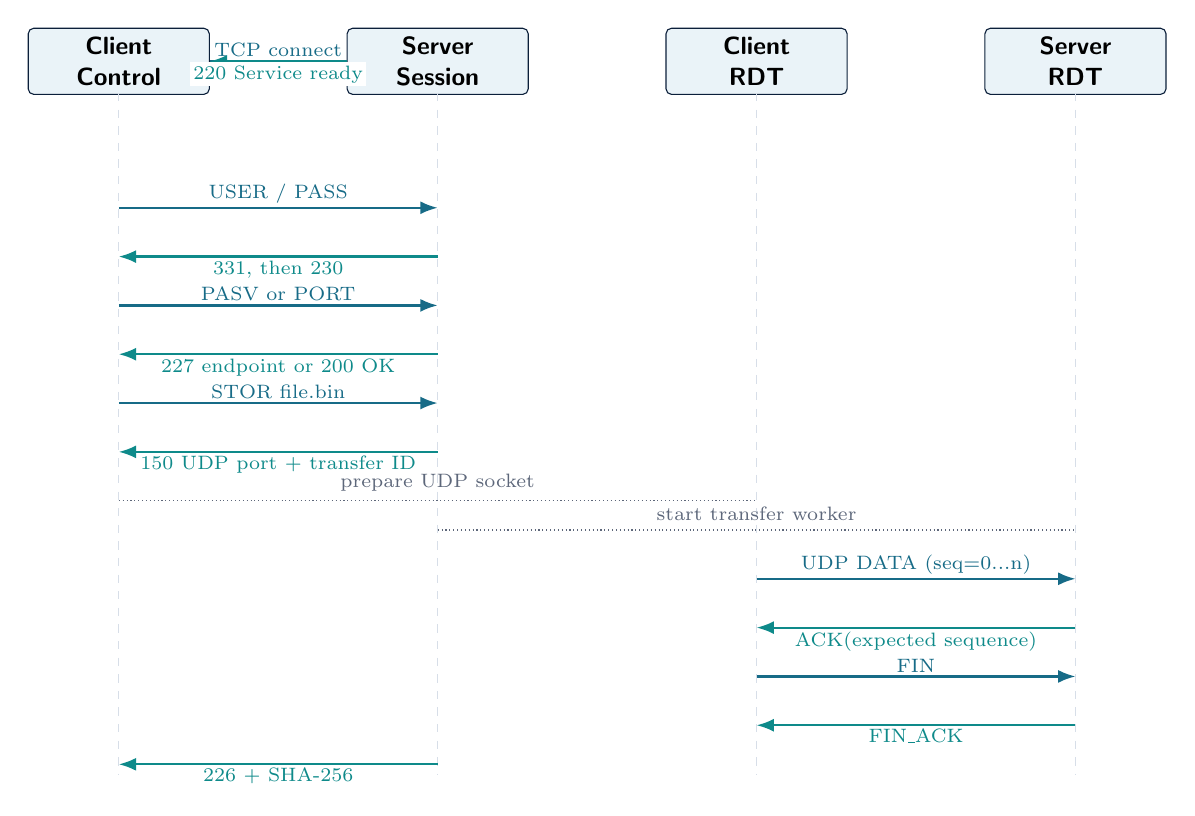
\begin{tikzpicture}[x=0.9cm,y=0.62cm]
  \node[actor] (cctrl) at (0,0) {Client\\Control};
  \node[actor] (session) at (4.5,0) {Server\\Session};
  \node[actor] (crdt) at (9,0) {Client\\RDT};
  \node[actor] (srdt) at (13.5,0) {Server\\RDT};
  \foreach \x in {0,4.5,9,13.5} {\draw[lifeline] (\x,-0.65) -- (\x,-14.6);}
  \draw[line] (cctrl) -- node[midway,above,fill=white,inner sep=1.2pt,font=\scriptsize]{TCP connect} (session);
  \draw[returnline] (session) -- node[midway,below,fill=white,inner sep=1.2pt,font=\scriptsize]{220 Service ready} (cctrl);
  \draw[line] (0,-3.0) -- node[midway,above,fill=white,inner sep=1.2pt,font=\scriptsize]{USER / PASS} (4.5,-3.0);
  \draw[returnline] (4.5,-4.0) -- node[midway,below,fill=white,inner sep=1.2pt,font=\scriptsize]{331, then 230} (0,-4.0);
  \draw[line] (0,-5.0) -- node[midway,above,fill=white,inner sep=1.2pt,font=\scriptsize]{PASV or PORT} (4.5,-5.0);
  \draw[returnline] (4.5,-6.0) -- node[midway,below,fill=white,inner sep=1.2pt,font=\scriptsize]{227 endpoint or 200 OK} (0,-6.0);
  \draw[line] (0,-7.0) -- node[midway,above,fill=white,inner sep=1.2pt,font=\scriptsize]{STOR file.bin} (4.5,-7.0);
  \draw[returnline] (4.5,-8.0) -- node[midway,below,fill=white,inner sep=1.2pt,font=\scriptsize]{150 UDP port + transfer ID} (0,-8.0);
  \draw[densely dotted,color=InkMuted] (0,-9.0) -- node[midway,above,font=\scriptsize\color{InkMuted}]{prepare UDP socket} (9,-9.0);
  \draw[densely dotted,color=InkMuted] (4.5,-9.6) -- node[midway,above,font=\scriptsize\color{InkMuted}]{start transfer worker} (13.5,-9.6);
  \draw[line] (9,-10.6) -- node[midway,above,fill=white,inner sep=1.2pt,font=\scriptsize]{UDP DATA (seq=0...n)} (13.5,-10.6);
  \draw[returnline] (13.5,-11.6) -- node[midway,below,fill=white,inner sep=1.2pt,font=\scriptsize]{ACK(expected sequence)} (9,-11.6);
  \draw[line] (9,-12.6) -- node[midway,above,fill=white,inner sep=1.2pt,font=\scriptsize]{FIN} (13.5,-12.6);
  \draw[returnline] (13.5,-13.6) -- node[midway,below,fill=white,inner sep=1.2pt,font=\scriptsize]{FIN\_ACK} (9,-13.6);
  \draw[returnline] (4.5,-14.4) -- node[midway,below,fill=white,inner sep=1.2pt,font=\scriptsize]{226 + SHA-256} (0,-14.4);
\end{tikzpicture}
\caption{Full upload lifecycle. For \code{RETR}, the RDT sender is the server and the DATA/ACK direction is reversed.}
\label{fig:lifecycle}
\end{figure}

\subsection{Interaction Rules}

\begin{itemize}
  \item Commands are UTF-8 text lines terminated by CRLF. The server returns FTP-style numeric responses such as \code{220}, \code{230}, \code{150}, \code{226}, and \code{426}.
  \item The preliminary \code{150} response includes a server UDP port and transfer identifier. The identifier isolates simultaneous transfers.
  \item A sender retransmits if a matching acknowledgement is not received before timeout. The receiver writes only the next expected DATA sequence number.
  \item Transfer completion requires FIN/FIN\_ACK and then a TCP \code{226 Transfer complete}; SHA-256 digest follows response.
  \item \code{ABOR} sets a cancellation event, closes active data/UDP sockets, returns \code{426}, and removes the temporary upload file rather than publishing partial data.
\end{itemize}

\section{Project-Wide Data Structures}

\subsection{TCP Control Packet Format}

The control protocol is intentionally line-oriented rather than binary. The parser normalizes command names to uppercase and limits an incoming line to 4096 bytes.

\begin{table}[htbp]
\centering
\begin{tabularx}{\textwidth}{@{}P{37mm}Y Y@{}}
\toprule
\textbf{Message} & \textbf{Wire format} & \textbf{Example} \\
\midrule
Client command & \code{COMMAND [SP argument] CRLF}; UTF-8 text & \code{STOR report.pdf\textbackslash r\textbackslash n} \\
Server reply & \code{DDD SP message CRLF}; \code{DDD} is a three-digit reply code & \code{226 Transfer complete}; SHA-256 digest follows \\
Parsed command object & \code{Command(name: str, argument: str | None)} & \code{Command("STOR", "report.pdf")} \\
\bottomrule
\end{tabularx}
\caption{TCP control-plane message representations.}
\end{table}

\subsection{Reliable UDP Header}

Each UDP datagram starts with a fixed 22-byte header encoded in network byte order with Python format \code{!2sBBIIIHI}. The checksum covers the header with a zeroed checksum field followed by the payload.

\begin{table}[htbp]
\centering
\begin{tabularx}{\textwidth}{@{}P{24mm}P{19mm}P{19mm}Y@{}}
\toprule
\textbf{Field} & \textbf{Bytes} & \textbf{Offset} & \textbf{Purpose} \\
\midrule
Magic & 2 & 0 & Constant \code{HF}; filters unrelated datagrams. \\
Version & 1 & 2 & Protocol version; current value is 1. \\
Flags & 1 & 3 & Bit flags: DATA=0x01, ACK=0x02, FIN=0x04, FIN\_ACK=0x08, ERROR=0x10. \\
Transfer ID & 4 & 4 & Unsigned 32-bit identifier that distinguishes concurrent transfers. \\
Sequence number & 4 & 8 & Zero-based DATA packet number. \\
ACK number & 4 & 12 & Sequence number being acknowledged. \\
Payload length & 2 & 16 & Payload size in bytes; maximum configured payload is 1024 bytes. \\
CRC-32 checksum & 4 & 18 & Detects corruption of the header and payload before processing. \\
Payload & 0--1024 & 22 & File bytes for DATA packets; normally empty for ACK and FIN control packets. \\
\bottomrule
\end{tabularx}
\caption{Custom reliable-UDP packet layout.}
\end{table}

\subsection{Session Management Structures}

The main per-client state is held in \code{ClientSession}. It is deliberately session-scoped to avoid sharing authentication, working-directory, or data-mode state between connected clients.

\begin{longtable}{@{}P{30mm}P{38mm}P{79mm}@{}}
\toprule
\textbf{State group} & \textbf{Representative fields} & \textbf{Responsibility} \\
\midrule
\endfirsthead
\toprule
\textbf{State group} & \textbf{Representative fields} & \textbf{Responsibility} \\
\midrule
\endhead
Identity and control & \code{\_conn}, \code{\_addr}, \code{\_config}, \code{\_log} & Own TCP socket, client address, configuration, and session logging callback. \\
Authentication & \code{\_auth\_state}, \code{\_pending\_username}, \code{\_username} & Enforce USER/PASS workflow and restrict post-login commands. \\
Filesystem context & \code{\_fm}, \code{\_cwd}, \code{\_rnfr\_path} & Map virtual FTP paths safely into the server storage root and support rename transactions. \\
Transfer configuration & \code{\_transfer\_type}, \code{\_data\_mode}, \code{\_active\_host}, \code{\_active\_port}, \code{\_pasv\_sock} & Keep TYPE and PORT/PASV setup independent for each client. \\
Transfer lifecycle & \code{\_transfer\_thread}, \code{\_transfer\_cancel}, \code{\_transfer\_sockets}, transfer ID counter & Run a transfer asynchronously, cancel it safely, close its sockets, and allocate identifiers. \\
Synchronization & \code{\_send\_lock}, \code{\_transfer\_lock} & Serialize control replies and protect transfer lifecycle state from worker/control-thread races. \\
Dispatch & \code{\_handlers} & Maps command names to handlers for authentication, files, directories, transfer, and help commands. \\
\bottomrule
\end{longtable}

\section{Functional Workflows}

\subsection{Server Thread-Dispatch Logic}

The server accepts TCP connections and creates one \code{ClientSession} thread per client. Each session validates and dispatches commands sequentially while transfer work executes in a dedicated worker thread.

\begin{figure}[H]
\centering
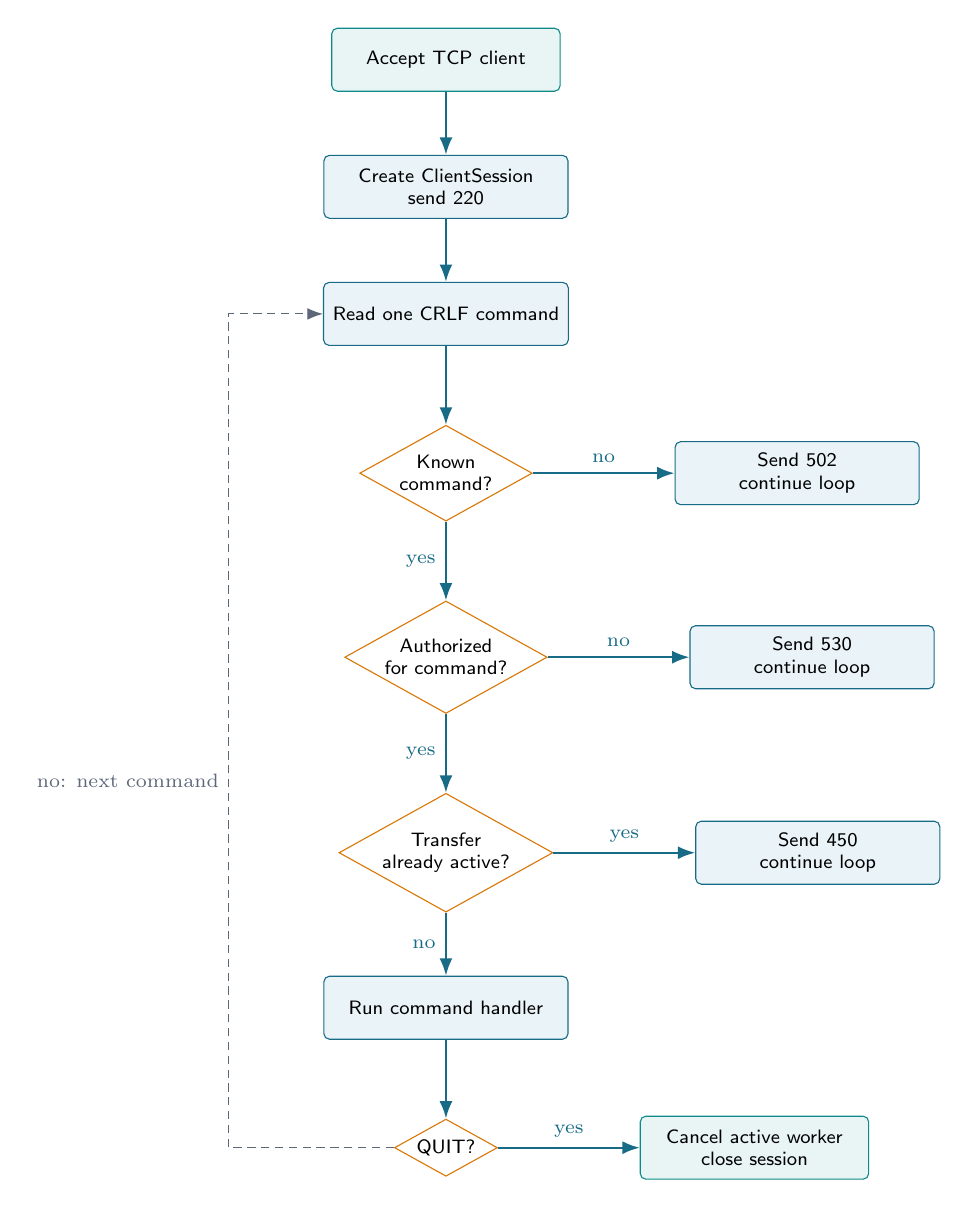
\begin{tikzpicture}[node distance=8mm]
  \node[state] (start) {Accept TCP client};
  \node[flow,below=of start] (session) {Create ClientSession\\send 220};
  \node[flow,below=of session] (read) {Read one CRLF command};
  \node[decision,below=of read,yshift=-2mm] (known) {Known\\command?};
  \node[flow,right=18mm of known] (err502) {Send 502\\continue loop};
  \node[decision,below=of known,yshift=-2mm] (auth) {Authorized\\for command?};
  \node[flow,right=18mm of auth] (err530) {Send 530\\continue loop};
  \node[decision,below=of auth,yshift=-2mm] (busy) {Transfer\\already active?};
  \node[flow,right=18mm of busy] (err450) {Send 450\\continue loop};
  \node[flow,below=of busy] (dispatch) {Run command handler};
  \node[decision,below=of dispatch,yshift=-2mm] (quit) {QUIT?};
  \node[state,right=18mm of quit] (end) {Cancel active worker\\close session};
  \draw[line] (start) -- (session);
  \draw[line] (session) -- (read);
  \draw[line] (read) -- (known);
  \draw[line] (known) -- node[left,font=\scriptsize]{yes} (auth);
  \draw[line] (known.east) -- node[above,font=\scriptsize]{no} (err502.west);
  \draw[line] (auth) -- node[left,font=\scriptsize]{yes} (busy);
  \draw[line] (auth.east) -- node[above,font=\scriptsize]{no} (err530.west);
  \draw[line] (busy) -- node[left,font=\scriptsize]{no} (dispatch);
  \draw[line] (busy.east) -- node[above,font=\scriptsize]{yes} (err450.west);
  \draw[line] (dispatch) -- (quit);
  \draw[line] (quit.east) -- node[above,font=\scriptsize]{yes} (end.west);
  \draw[densely dashed,-{Latex[length=2mm]},color=InkMuted] (quit.west) -- ++(-2.1,0) |- node[pos=0.22,left,font=\scriptsize]{no: next command} (read.west);
\end{tikzpicture}
\caption{Per-session command dispatch. Error branches explicitly continue the read loop; only the normal non-QUIT branch is drawn as a return path.}
\end{figure}

\subsection{Reliable UDP Sender and Receiver State Machines}

\begin{figure}[H]
\centering
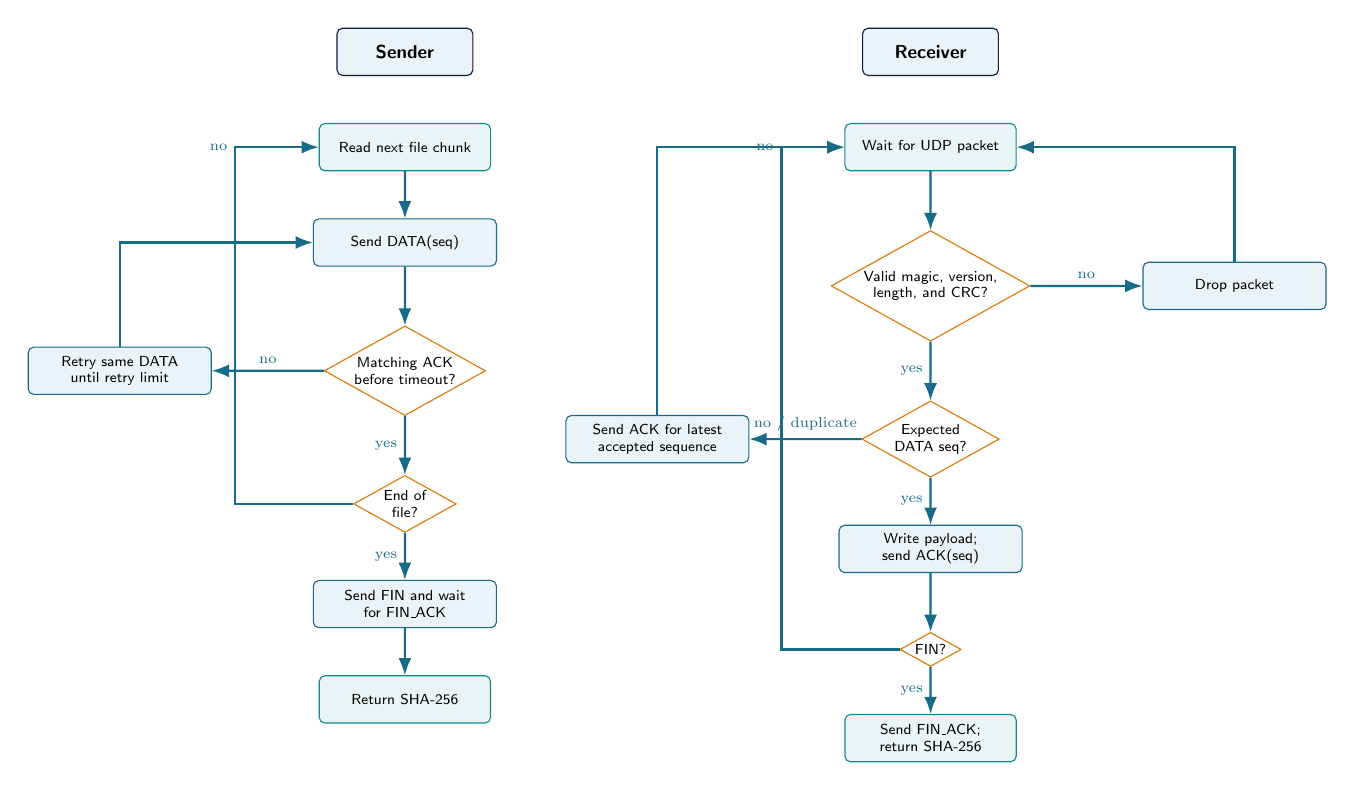
\begin{tikzpicture}[node distance=8mm,scale=0.75,transform shape]
  \node[actor] (senderTitle) at (-3.5,0) {Sender};
  \node[state,below=of senderTitle] (sread) {Read next file chunk};
  \node[flow,below=of sread] (ssend) {Send DATA(seq)};
  \node[decision,below=of ssend,yshift=-2mm] (sack) {Matching ACK\\before timeout?};
  \node[flow,left=of sack,xshift=-11mm] (sretry) {Retry same DATA\\until retry limit};
  \node[decision,below=of sack,yshift=-2mm] (seof) {End of\\file?};
  \node[flow,below=of seof] (sfin) {Send FIN and wait\\for FIN\_ACK};
  \node[state,below=of sfin] (sdone) {Return SHA-256};
  \draw[line] (sread) -- (ssend);
  \draw[line] (ssend) -- (sack);
  \draw[line] (sack) -- node[above,font=\scriptsize]{no} (sretry);
  \draw[line] (sretry) |- (ssend.west);
  \draw[line] (sack) -- node[left,font=\scriptsize]{yes} (seof);
  \draw[line] (seof.west) -| ++(-2.0,0) |- node[left,font=\scriptsize]{no} (sread.west);
  \draw[line] (seof) -- node[left,font=\scriptsize]{yes} (sfin);
  \draw[line] (sfin) -- (sdone);

  \node[actor] (receiverTitle) at (5.4,0) {Receiver};
  \node[state,below=of receiverTitle] (rwait) {Wait for UDP packet};
  \node[decision,below=of rwait,yshift=-2mm] (rvalid) {Valid magic, version,\\length, and CRC?};
  \node[flow,right=of rvalid,xshift=11mm] (rdrop) {Drop packet};
  \node[decision,below=of rvalid,yshift=-2mm] (rdata) {Expected\\DATA seq?};
  \node[flow,below=of rdata] (rwrite) {Write payload;\\send ACK(seq)};
  \node[flow,left=of rdata,xshift=-11mm] (rackdup) {Send ACK for latest\\accepted sequence};
  \node[decision,below=of rwrite,yshift=-2mm] (rfin) {FIN?};
  \node[state,below=of rfin] (rdone) {Send FIN\_ACK;\\return SHA-256};
  \draw[line] (rwait) -- (rvalid);
  \draw[line] (rvalid) -- node[above,font=\scriptsize]{no} (rdrop);
  \draw[line] (rdrop) |- (rwait.east);
  \draw[line] (rvalid) -- node[left,font=\scriptsize]{yes} (rdata);
  \draw[line] (rdata) -- node[left,font=\scriptsize]{yes} (rwrite);
  \draw[line] (rdata) -- node[above,font=\scriptsize]{no / duplicate} (rackdup);
  \draw[line] (rackdup) |- (rwait.west);
  \draw[line] (rwrite) -- (rfin);
  \draw[line] (rfin.west) -| ++(-2.0,0) |- node[left,font=\scriptsize]{no} (rwait.west);
  \draw[line] (rfin) -- node[left,font=\scriptsize]{yes} (rdone);
\end{tikzpicture}
\caption{Stop-and-Wait sender and receiver state machines. Cancellation is checked inside transfer/wait loops and terminates the active worker.}
\end{figure}

\subsection{Active/Passive Mode Selection}

\begin{figure}[H]
\centering
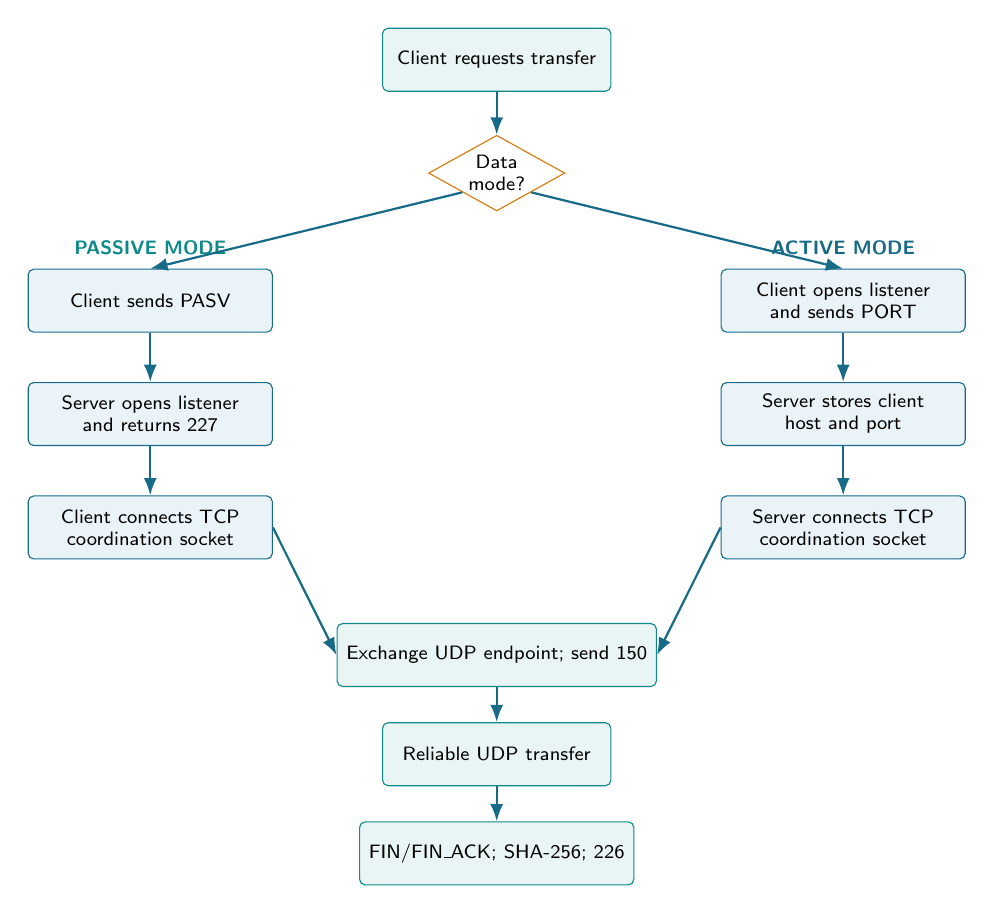
\begin{tikzpicture}[x=1cm,y=0.9cm]
  \node[state] (begin) at (0,0) {Client requests transfer};
  \node[decision] (mode) at (0,-1.6) {Data\\mode?};
  \node[font=\sffamily\scriptsize\bfseries\color{Teal}] at (-4.4,-2.65) {PASSIVE MODE};
  \node[flow] (pasv1) at (-4.4,-3.4) {Client sends PASV};
  \node[flow] (pasv2) at (-4.4,-5.0) {Server opens listener\\and returns 227};
  \node[flow] (pasv3) at (-4.4,-6.6) {Client connects TCP\\coordination socket};
  \node[font=\sffamily\scriptsize\bfseries\color{Blue}] at (4.4,-2.65) {ACTIVE MODE};
  \node[flow] (port1) at (4.4,-3.4) {Client opens listener\\and sends PORT};
  \node[flow] (port2) at (4.4,-5.0) {Server stores client\\host and port};
  \node[flow] (port3) at (4.4,-6.6) {Server connects TCP\\coordination socket};
  \node[state] (merge) at (0,-8.4) {Exchange UDP endpoint; send 150};
  \node[state] (udp) at (0,-9.8) {Reliable UDP transfer};
  \node[state] (complete) at (0,-11.2) {FIN/FIN\_ACK; SHA-256; 226};
  \draw[line] (begin) -- (mode);
  \draw[line] (mode.south west) -- (pasv1.north);
  \draw[line] (pasv1) -- (pasv2);
  \draw[line] (pasv2) -- (pasv3);
  \draw[line] (mode.south east) -- (port1.north);
  \draw[line] (port1) -- (port2);
  \draw[line] (port2) -- (port3);
  \draw[line] (pasv3.east) -- (merge.west);
  \draw[line] (port3.west) -- (merge.east);
  \draw[line] (merge) -- (udp);
  \draw[line] (udp) -- (complete);
\end{tikzpicture}
\caption{Passive and active data coordination. Both modes use the same reliable UDP payload protocol after setup.}
\end{figure}

\clearpage
\section{Task Assignment Matrix}


\begin{longtable}{@{}P{23mm}P{25mm}P{25mm}P{74mm}@{}}
\toprule
\textbf{Engineering component} & \textbf{Primary owner} & \textbf{Collaborator} & \textbf{Responsibilities and defense topics} \\
\midrule
\endfirsthead
\toprule
\textbf{Engineering component} & \textbf{Primary owner} & \textbf{Collaborator} & \textbf{Responsibilities and defense topics} \\
\midrule
\endhead
Architecture and protocol design & Vinh Thuan &  & TCP/UDP separation, FTP reply semantics, packet layout, and protocol sequence diagrams. \\
Common module & Vinh Thuan & Minh Khoa & \code{common/}: configuration, command parsing, reply formatting, CRC-32, SHA-256, UDP codec. \\
Reliable UDP transport & Minh Khoa &  & \code{transport/}: Stop-and-Wait, ACK, retry, duplicate and ordering behavior, FIN handshake, cancellation checks. \\
Server and session management & Vinh Thuan &  & \code{server/}: listen/accept, per-client threads, authentication, virtual paths, commands, transfer worker, ABOR. \\
Client and CLI & Minh Khoa &  & \code{client/}: REPL, command mapping, PASV/PORT setup, upload/download, digest comparison. \\
Testing and quality assurance & Minh Khoa & Vinh Thuan & Unit/integration tests; packet loss/reorder simulation; active transfer, ABOR, concurrency, and regression test evidence. \\
Documentation and demo & Vinh Thuan & Minh Khoa & Report, diagrams, screenshots, command transcript, live defense preparation, and repository traceability. \\
\bottomrule
\end{longtable}

\section{Self-Assessment \& Peer Evaluation}

The contribution split below is derived from the ownership recorded in Section~4. Both members own three core engineering areas, with shared responsibility for the common module; a 50\% / 50\% distribution is therefore consistent with the documented scope of work.

\begin{longtable}{@{}P{30mm}P{23mm}P{93mm}@{}}
\toprule
\textbf{Member} & \textbf{Contribution} & \textbf{Self-assessment} \\
\midrule
\endfirsthead
\toprule
\textbf{Member} & \textbf{Contribution} & \textbf{Self-assessment} \\
\midrule
\endhead
Le Vinh Thuan & 50\% & I was responsible for the application architecture and protocol design, the server and session-management layer, and the documentation and demo materials. I can explain the TCP control-channel workflow, FTP-style replies, session lifecycle, path and command handling, transfer-worker dispatch, and the rationale behind the TCP/UDP split. I also collaborated on the common module, including the shared protocol and integrity utilities. \\
\addlinespace
Nguyen Minh Khoa & 50\% & I was responsible for the reliable UDP transport, the client and CLI workflow, and testing and quality assurance. I can explain Stop-and-Wait sequencing, acknowledgements, retransmission, duplicate/out-of-order handling, FIN completion, cancellation, active/passive coordination, and SHA-256 verification. I also collaborated on the common module and prepared regression evidence for loss, reordering, concurrent sessions, and transfer cancellation. \\
\midrule
\textbf{Total} & \textbf{100\%} &  \\
\bottomrule
\end{longtable}

\section{GenAI Usage \& Code Refinement Log}

You can view the GenAI Usage on the Prompt.md file

\section{Application Demo Evidence}

\subsection{Recorded CLI Transcript and Hash Comparison}

The following transcript was captured from a local server at \code{127.0.0.1:2121}. The same SHA-256 value was returned after upload, by the remote \code{HASH} command, and after download.

\begin{lstlisting}
ftp> connect
Connected to 127.0.0.1:2121 - Hybrid FTP Server ready
ftp> login admin 1234
Logged in.
ftp> put sample.txt demo-sample.txt
Upload complete. SHA-256: f84e951432fc2c1b6da5f28397ed07d6c362098a4a7b92848eafbda1770a8b76
ftp> hash demo-sample.txt
f84e951432fc2c1b6da5f28397ed07d6c362098a4a7b92848eafbda1770a8b76
ftp> get demo-sample.txt demo-sample.txt
Download complete. SHA-256: f84e951432fc2c1b6da5f28397ed07d6c362098a4a7b92848eafbda1770a8b76
ftp> dele demo-sample.txt
Deleted 'demo-sample.txt'.
ftp> quit
Disconnected.
\end{lstlisting}

\subsection{Captured Runtime Evidence}

The following uncropped terminal captures provide direct runtime evidence for the core upload path, active-mode binary transfer, and concurrent session handling.

\begin{figure}[H]
  \centering
  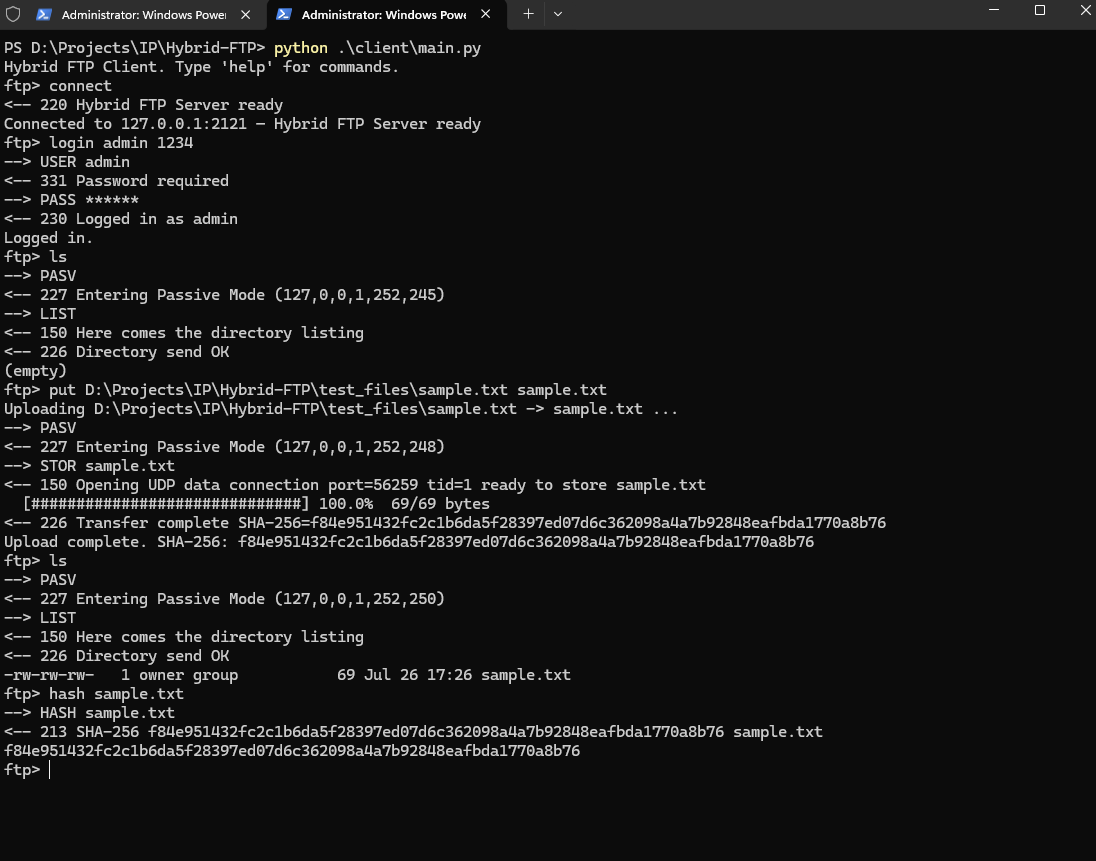
\includegraphics[width=\textwidth,height=0.76\textheight,keepaspectratio]{figures/BasicUpload.png}
  \caption{Basic passive-mode upload. The client trace shows TCP connection and login, PASV coordination, STOR, the 150 readiness reply, the 226 completion reply, and the resulting SHA-256 digest.}
  \label{fig:basic-upload}
\end{figure}

\begin{figure}[H]
  \centering
  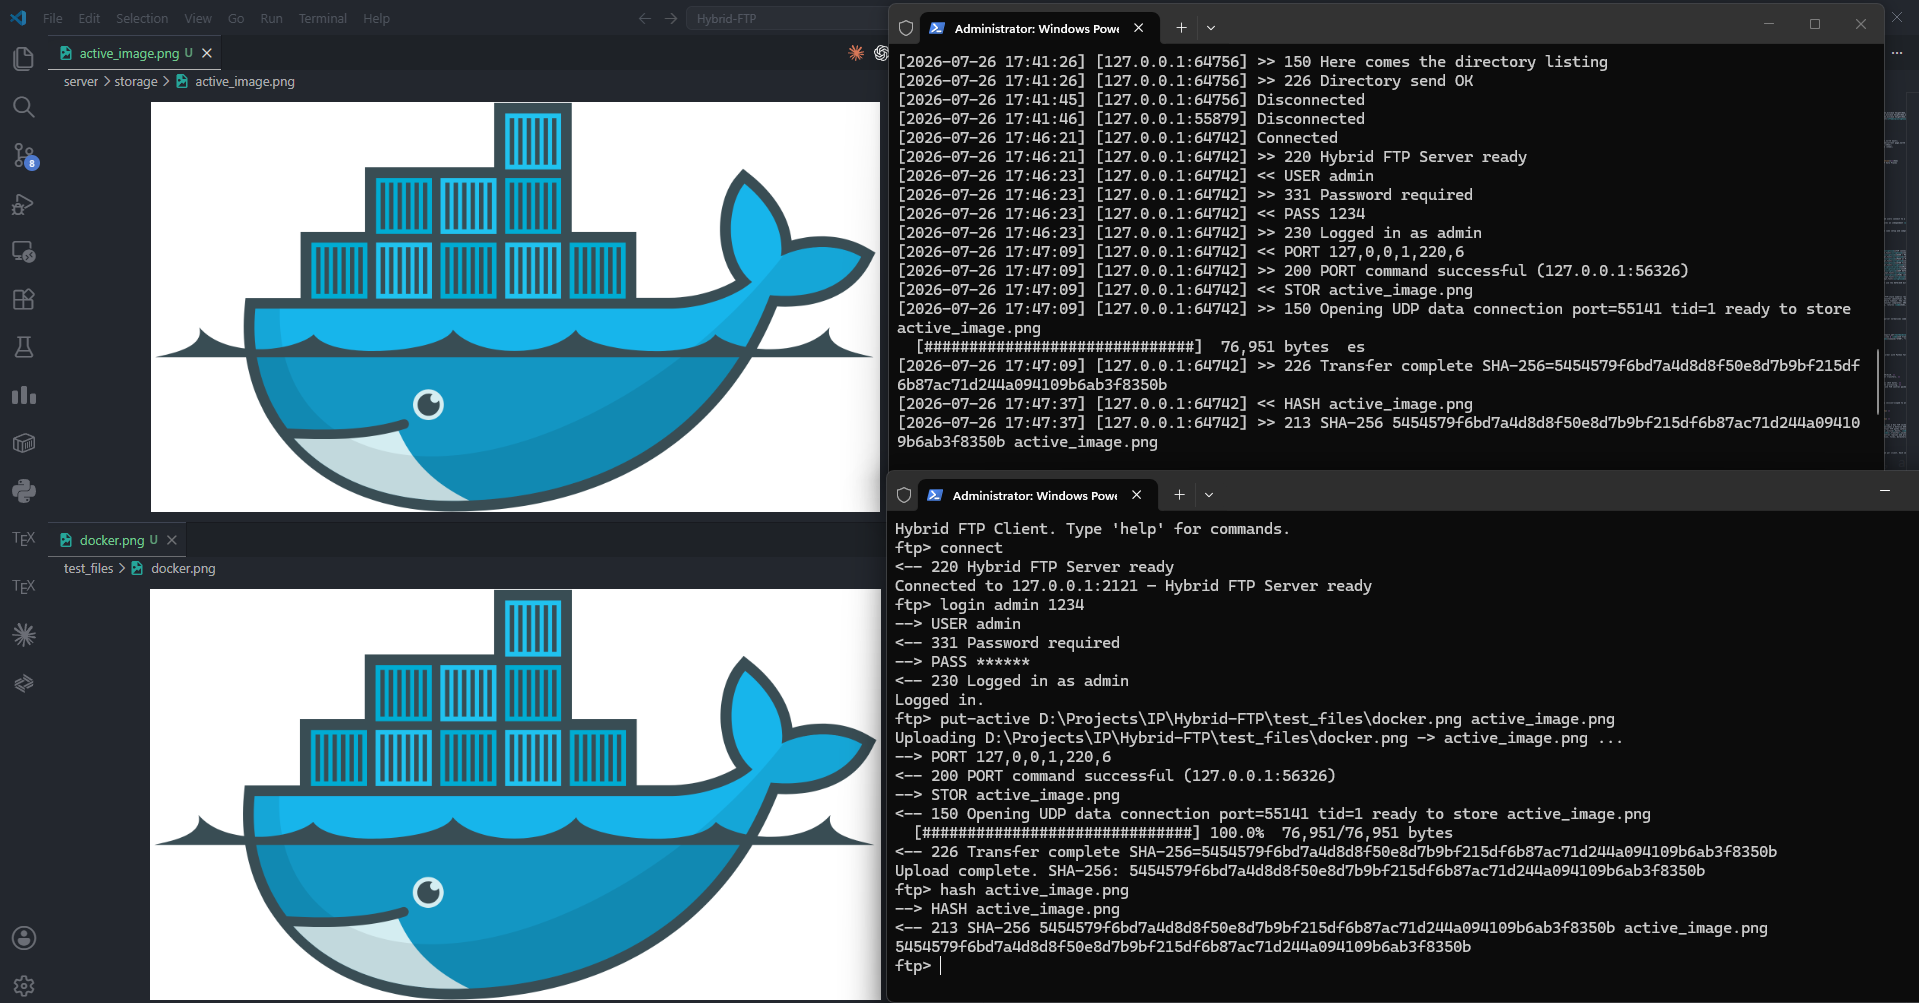
\includegraphics[width=\textwidth,height=0.76\textheight,keepaspectratio]{figures/ActiveUpload.png}
  \caption{Active-mode upload of an image file (binary payload). The trace uses PORT coordination before STOR and completes the reliable UDP transfer with a SHA-256 digest, demonstrating that the active path preserves binary data integrity.}
  \label{fig:active-binary-upload}
\end{figure}

\begin{figure}[H]
  \centering
  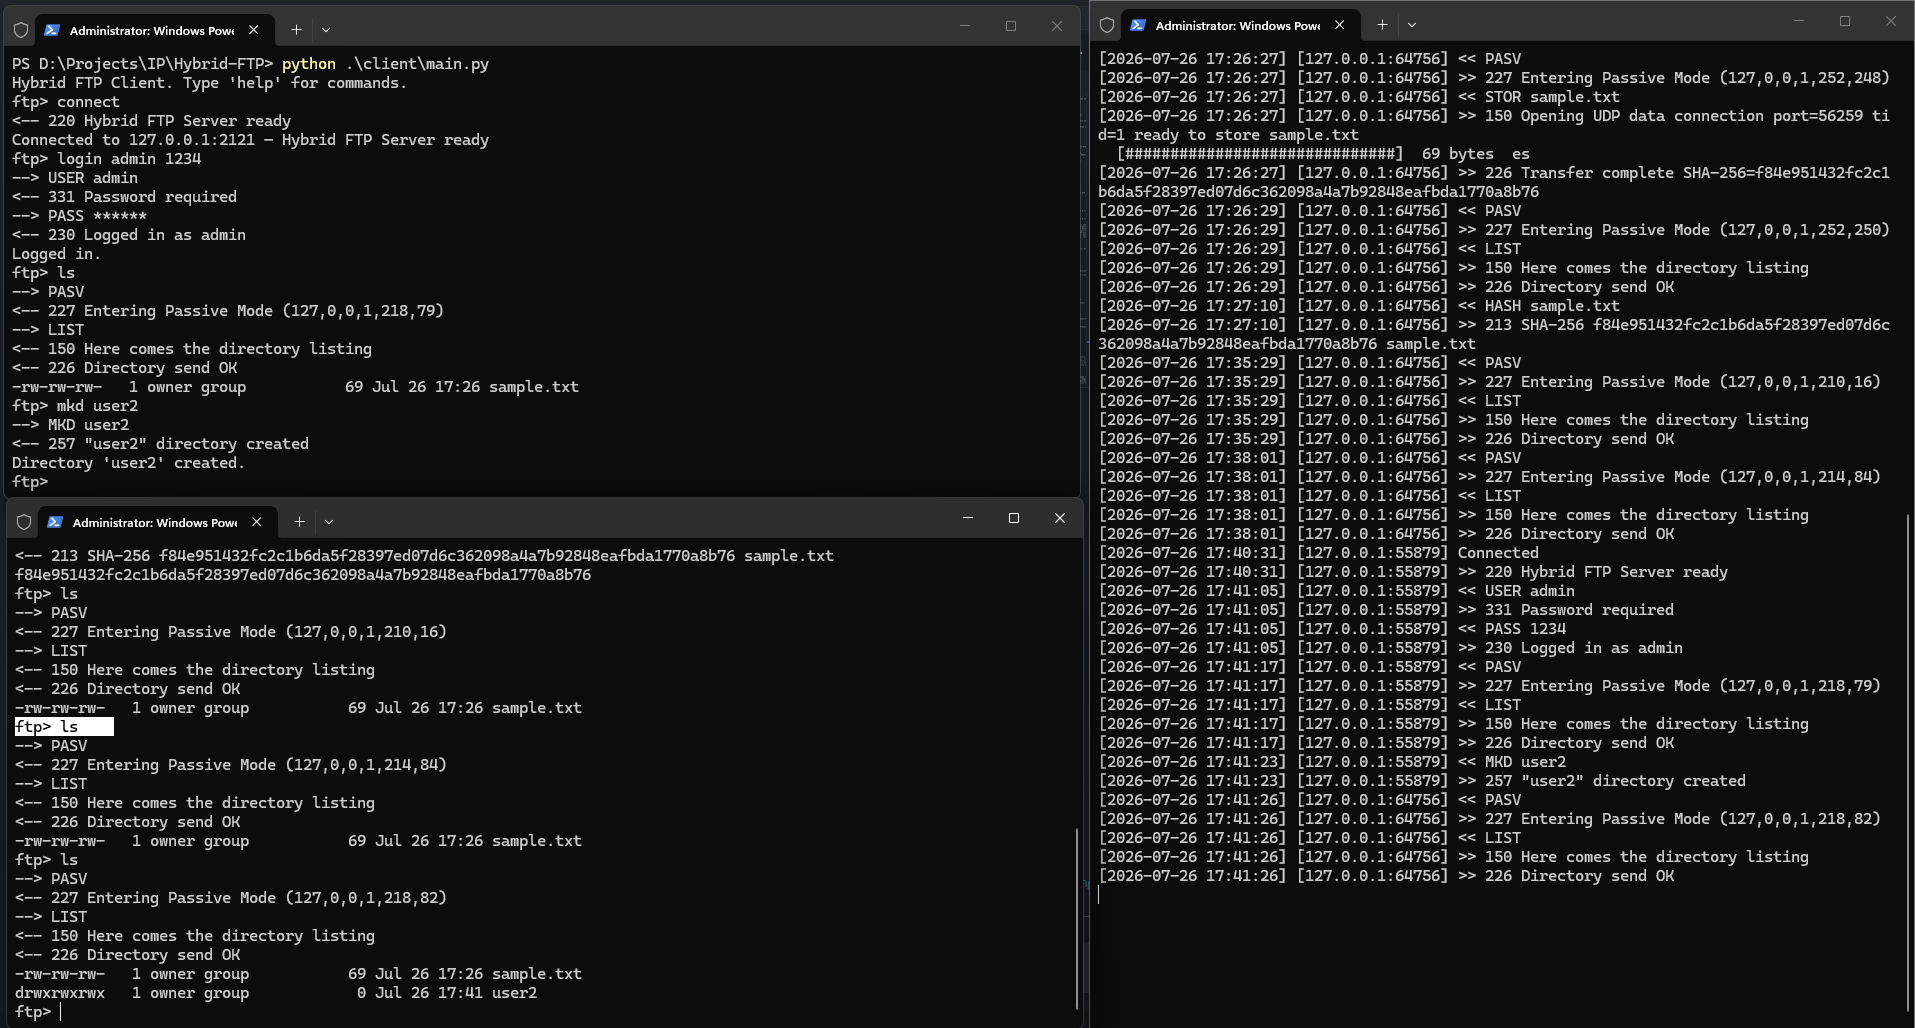
\includegraphics[width=\textwidth,height=0.76\textheight,keepaspectratio]{figures/Concurence.png}
  \caption{Concurrent-session evidence. Two client connections remain active simultaneously, with distinct client endpoints/session activity recorded by the server.}
  \label{fig:concurrent-sessions}
\end{figure}


% \begin{thebibliography}{9}
% \bibitem{rfc959}
% J. Postel and J. Reynolds. \textit{File Transfer Protocol}. RFC 959, October 1985.
% \bibitem{projectrepo}
% Hybrid FTP project repository: source modules under \code{common/}, \code{transport/}, \code{server/}, \code{client/}, and \code{test/}; project documentation under \code{docs/}.
% \end{thebibliography}

\end{document}
